\documentclass[10pt,xcolor=pdflatex]{beamer}
\usepackage{newcent}
\usepackage[utf8]{inputenc}
\usepackage[czech]{babel}
\usepackage{hyperref}
\usepackage{textpos}
\usepackage{multicol}
\usepackage{tikz}
\usepackage{fancyvrb}
\usepackage{color}
\usepackage{subfig}
\usepackage{geometry}
\usepackage{graphicx}
\usepackage{epstopdf}
\usepackage{todonotes}

\makeatletter
\g@addto@macro{\UrlBreaks}{\UrlOrds}
\makeatother

\newcommand{\itab}[1]{\hspace{0em}\rlap{#1}}
\newcommand{\tab}[1]{\hspace{.15\textwidth}\rlap{#1}}
\newcommand{\putat}[3]{\begin{picture}(0,0)(0,0)\put(#1,#2){#3}\end{picture}}

\epstopdfDeclareGraphicsRule{.gif}{png}{.png}{convert gif:#1 png:\OutputFile}
\AppendGraphicsExtensions{.gif}
\usetheme{FIT}

\def\uv#1{\quotedblbase#1\textquotedblleft}%

%%%%%%%%%%%%%%%%%%%%%%%%%%%%%%%%%%%%%%%%%%%%%%%%%%%%%%%%%%%%%%%%%%
\title[GJA 4]{EJB and JavaServer Faces}

\author[]{Jaroslav Dytrych}

\institute[]{Faculty of Information Technology
Brno University of Technology \\
Bo\v{z}et\v{e}chova 1/2. 612 66 Brno - Kr\'alovo Pole\\
dytrych@fit.vutbr.cz}

\date{10 October 2023}
%\date{\today}
%\date{} % bez data

%%%%%%%%%%%%%%%%%%%%%%%%%%%%%%%%%%%%%%%%%%%%%%%%%%%%%%%%%%%%%%%%%%

\begin{document}

\frame[plain]{\titlepage}

\bluepage{EJB (Enterprise Java Beans)}

\begin{frame}[fragile]\frametitle{Contents}
	\begin{itemize}
		\item EJB Introduction
    	\item Session Beans
    	\item Message Driven Beans (based on JMS)
    	\item Transactions
    	\item Deployment
    	\item New features in EJB 3.1
	\end{itemize}
\end{frame}


\begin{frame}\frametitle{EJB}
	\begin{itemize}
      \item Enterprise JavaBeans (EJB)
        \begin{itemize}
          \item Enterprise bean is a server-side component that encapsulates the business logic of an application.
          \item EJB execute within an EJB container, which is running in the EJB server.
        \end{itemize}
	\end{itemize}
\begin{tikzpicture}[remember picture,overlay]
    \node[xshift=-0.6cm,yshift=-1.3cm] at (current page.north east){%
    
\includegraphics[width=1cm]{img/pozor}};
\end{tikzpicture}
\end{frame}


\begin{frame}\frametitle{EJB server}
	\begin{itemize}
		\item EJB server is a part of an application server that hosts EJB containers
          \begin{itemize}
            \item can be also standalone (Apache TomEE)
          \end{itemize}
		\item EJBs do not interact directly with the EJB server.
		\item GlassFish (Oracle), WebSphere (IBM), WebLogic (Oracle), WildFly (Red Hat), WebObjects (Apple), \ldots
		\item EJB specification outlines eight services that must be provided by an EJB server:
        \begin{itemize}
        	\item Naming
        	\item Transaction
        	\item Security
        	\item Persistence
        	\item Concurrency
        	\item Life cycle
        	\item Messaging
        	\item Timer 
        \end{itemize}
	\end{itemize}
\begin{tikzpicture}[remember picture,overlay]
    \node[xshift=-0.6cm,yshift=-1.3cm] at (current page.north east){%
    
\includegraphics[width=1cm]{img/lupa}};
\end{tikzpicture}
\end{frame}


\begin{frame}\frametitle{EJB Container}
	\begin{itemize}
		\item EJB Container is a runtime environment for EJB component beans.
		\item Containers are transparent to the client.
          \begin{itemize}
            \item There is no client API to manipulate the container.
          \end{itemize}
		\item Container provides EJB instance life cycle management and EJB instance identification.
		\item Container manages the connections to the enterprise information systems (EISs). % EIS Tier
		\item Container provides services, such as transaction management, concurrency control, pooling (cache with~beans) and security authorization.
	\end{itemize}
\begin{tikzpicture}[remember picture,overlay]
    \node[xshift=-0.6cm,yshift=-1.3cm] at (current page.north east){%
    
\includegraphics[width=1cm]{img/pozor}};
\end{tikzpicture}
\end{frame}


\begin{frame}\frametitle{Multitiered Java EE Applications}
\begin{center}
  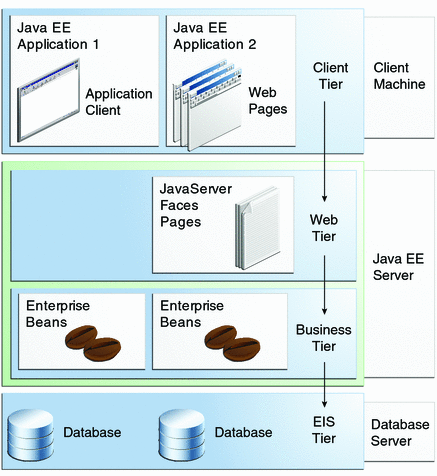
\includegraphics[scale=0.49]{img/overview-multitieredapps}
\end{center}
\end{frame}


\begin{frame}\frametitle{EJB Components}
	\begin{itemize}
		\item EJB components are server-side, modular, reusable, and containing specific units of functionality.
		\item They are similar to the Java classes as we create every day, but are subject to special restrictions and must provide specific interfaces for container and client use and access.
		\item We should consider using EJB components for applications that require scalability, transactional processing, or~availability to multiple client types.
	\end{itemize}
\end{frame}


\begin{frame}\frametitle{Enterprise Java Bean types}
	\begin{itemize}
		\item Session Beans
          \begin{itemize}
        	\item models task or workflow
        	\item Façade for Entity beans
              \begin{itemize}
                \item structural design pattern -- simplified interface to a larger set of~interfaces.
              \end{itemize}
        	\item maintains conversational state with clients (one bean per client)
          \end{itemize}
		\item Message Driven Beans
          \begin{itemize}
        	\item asynchronous communication with MOM (Message Oriented Middleware) -- distributed over heterogeneous platforms
        	\item allows non-Java EE resources to access Session and Entity Beans via JCA (Java EE Connector Architecture -- connects AS with EIS) Resource adapters
            \item uses JMS
          \end{itemize}
        \item (Entity Beans 2.1) JPA 2.0 in Java EE 6
          \begin{itemize}
            \item implicitly persistent
        	\item transparent persistence with transaction support
        	\item typically stored in a relational database (Object/Relational Mapping) 
          \end{itemize}
	\end{itemize}
\begin{textblock}{15}(8.3,0.3)
    {\footnotesize Example guestbook-jee6 (Entity)}
\end{textblock}
\begin{tikzpicture}[remember picture,overlay]
    \node[xshift=-0.6cm,yshift=-1.3cm] at (current page.north east){%
    
\includegraphics[width=1cm]{img/pozor}};
\end{tikzpicture}
\end{frame}


\begin{frame}\frametitle{Stateless Session Beans}
	\begin{itemize}
		\item \texttt{@Stateless} annotation
		\item State only for the duration of a client invocation of a single method.
        \item Pool of stateless beans is managed by the container.
		\item Any available stateless session bean may handle the client request.
		\item Lifecycle event callbacks supported for stateless session beans (optional)
          \begin{itemize}
        	\item \texttt{@PostConstruct} -- occurs before the first business method invocation on the bean.
        	\item \texttt{@PreDestroy} -- occurs at the time the bean instance is destroyed.
          \end{itemize}
	\end{itemize}
\begin{tikzpicture}[remember picture,overlay]
    \node[xshift=-0.6cm,yshift=-1.3cm] at (current page.north east){%
    
\includegraphics[width=1cm]{img/pozor}};
\end{tikzpicture}
\end{frame}


\begin{frame}[fragile]\frametitle{Stateless Session Beans}
  \begin{verbatim}
  @Stateless
  public class FooBean {
    @PostConstruct
    private void init() {...}

    @Remove
    public void remove() {}  // removed from container
  }
  \end{verbatim}
  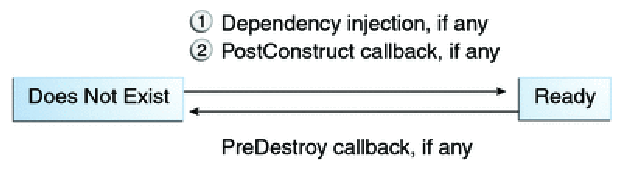
\includegraphics[scale=0.6]{img/obr1}
\begin{textblock}{10}(10.0,0.7)
    {\footnotesize Example StatelessBean}
\end{textblock}
\end{frame}


\begin{frame}\frametitle{Stateful Session Beans}
	\begin{itemize}
		\item Instance variables unique to the client/session.
		\item State is retained for the duration of the client/bean session.
		\item Client initiate creation and destruction (or timeout).
		\item Stateful Session Beans can not be pooled.
		\item Stateful Session Beans can be passivated.
		\item Supports following callbacks for the lifecycle events:
          \begin{itemize}
            \item \texttt{@PostConstruct} -- same as stateless bean, once for each session.
        	\item \texttt{@Init} -- designates the initialization method of a bean.
        	\item \texttt{@PreDestroy} -- same as stateless, once for each session.
        	\item \texttt{@PrePassivate} -- container invokes this method right before it passivates a stateful session bean (clean up held resources, such as database connections or any resources that cannot be transparently passivated using object serialization).
        	\item \texttt{@PostActivate} -- container invokes this method right after it reactivates the bean.
        	\item \texttt{@Remove} -- called by container before it ends the life of the stateful session bean. Than invokes the bean’s \texttt{PreDestroy} method, if any.
            \item \texttt{@AroundInvoke} -- interceptor method that interposes on~business methods (one per class).
          \end{itemize}
	\end{itemize}
\begin{tikzpicture}[remember picture,overlay]
    \node[xshift=-0.6cm,yshift=-1.3cm] at (current page.north east){%
    
\includegraphics[width=1cm]{img/pozor}};
\end{tikzpicture}
\end{frame}


\begin{frame}[fragile]\frametitle{Stateful Session Beans}
\begin{small}
	\begin{verbatim}
@Stateful
public class FooBean {
  @PostConstruct
  private void init() {...}

  @Remove
  public void remove() {}
}
	\end{verbatim}\end{small}
	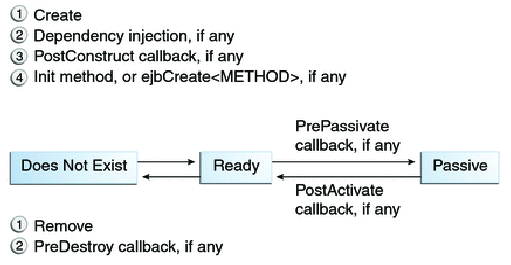
\includegraphics[scale=0.7]{img/obr2}
\begin{textblock}{10}(10.0,-0.6)
    {\footnotesize Example StatefullBean}
\end{textblock}
\end{frame}


\begin{frame}[fragile]\frametitle{Singleton Session Beans}
	\begin{itemize}
		\item Singleton Session Bean is a POJOs marked with \texttt{@Singleton} annotation,
		\item has only a single instance per JVM,
		\item supports data sharing and concurrent access,
		\item allows to set order of initialization (\texttt{@DependsOn}),
		\item initialization can be eager (\texttt{@Startup}).
		\item[]
        	\medskip
        	\begin{verbatim}
@Startup
@Singleton(name = "PrimaryBean")
@DependsOn("SecondaryBean")
public class PrimaryBean {…}

@Startup
@Singleton(name = "SecondaryBean")
public class SecondaryBean {…}
			\end{verbatim}
	\end{itemize}
\begin{tikzpicture}[remember picture,overlay]
    \node[xshift=-0.6cm,yshift=-1.3cm] at (current page.north east){%
    
\includegraphics[width=0.7cm]{img/pozor}};
\end{tikzpicture}
\end{frame}


\begin{frame}\frametitle{Business interfaces}
	\begin{itemize}
      \item Business interfaces
        \begin{itemize}
          \item visible to the client
          \item implemented inside the bean
        \end{itemize}
	\end{itemize}
\end{frame}


\begin{frame}\frametitle{Local and Remote Interface}
	\begin{itemize}
		\item Local Interface (\texttt{@Local})
          \begin{itemize}
            \item invoking EJBs within the same JVM,
            \item faster, but not so flexible, scalable and adaptable,
            \item no network traffic,
            \item parameters passed by reference.
          \end{itemize}
		\item Remote Interface (\texttt{@Remote})
          \begin{itemize}
        	\item invoking EJBs across JVMs,
        	\item anywhere on the network,
        	\item parameters passed by value (serialization/de-serialization).
          \end{itemize}
	\end{itemize}
\begin{tikzpicture}[remember picture,overlay]
    \node[xshift=-0.6cm,yshift=-1.3cm] at (current page.north east){%
    
\includegraphics[width=1cm]{img/pozor}};
\end{tikzpicture}
\end{frame}


\begin{frame}[fragile]\frametitle{Local and Remote Interface}
\begin{Verbatim}[fontsize=\footnotesize, commandchars=\\\{\}]
@Stateless
\textcolor{purple}{\textbf{public class}} CalculatorBean 
  \textcolor{purple}{\textbf{implements}} CalculatorRemote, CalculatorLocal \{
    \textcolor{purple}{\textbf{public int}} add(\textcolor{purple}{\textbf{int}} x, \textcolor{purple}{\textbf{int}} y) \{
        \textcolor{purple}{\textbf{return}} x + y;
    \}
    \textcolor{purple}{\textbf{public int}} subtract(\textcolor{purple}{\textbf{int}} x, \textcolor{purple}{\textbf{int}} y) \{
        \textcolor{purple}{\textbf{return}} x - y;
    \}
\}
\textcolor{purple}{\textbf{public interface}} Calculator \{
    \textcolor{purple}{\textbf{int}} add(\textcolor{purple}{\textbf{int}} x, \textcolor{purple}{\textbf{int}} y);
    \textcolor{purple}{\textbf{int}} subtract(\textcolor{purple}{\textbf{int}} x, \textcolor{purple}{\textbf{int}} y);
\}

@Remote
\textcolor{purple}{\textbf{public interface}} CalculatorRemote \textcolor{purple}{\textbf{extends}} Calculator \{\}
@Local
\textcolor{purple}{\textbf{public interface}} CalculatorLocal \textcolor{purple}{\textbf{extends}} Calculator \{\}
\end{Verbatim}
\end{frame}


\begin{frame}[fragile]\frametitle{No-interface view}
	\begin{itemize}
		\item New in EJB 3.1
		\item EJB may not have business interface.
		\item Session Beans are simple POJO.
		\item Automatically exposes public methods.
        \item[] \begin{Verbatim}[fontsize=\footnotesize, commandchars=\\\{\}]
@Stateless
\textcolor{purple}{\textbf{public class}} FooBean \{ 
    \textcolor{purple}{\textbf{public void}} foo() \{\ldots\}
\}
				\end{Verbatim}
        \item It is not necessary to use \texttt{@local} or \texttt{@remote} (selected automatically).
	\end{itemize}
\begin{tikzpicture}[remember picture,overlay]
    \node[xshift=-0.6cm,yshift=-1.3cm] at (current page.north east){%
    
\includegraphics[width=1cm]{img/pozor}};
\end{tikzpicture}
\end{frame}


\begin{frame}\frametitle{Message Driven EJB}
	\begin{itemize}
		\item \texttt{@MessageDriven} annotation
		\item invoked asynchronously by messages from standard Session Beans,
		\item cannot be invoked with local or remote interfaces (from clients),
		\item stateless, transaction aware,
		\item JMS (Java Messaging Service) used as a transport layer,
		\item implements method \texttt{onMessage(\ldots)}.
		\item Two types of messaging:
          \begin{itemize}
        	\item point-to-point (queues)
        	\item pub-sub (topics)
          \end{itemize}
	\end{itemize}
\begin{textblock}{10}(7.2,2.6)
    {\footnotesize Example MessageDrivenBean (JDK 1.8)}
\end{textblock}
\begin{tikzpicture}[remember picture,overlay]
    \node[xshift=-0.6cm,yshift=-1.3cm] at (current page.north east){%
    
\includegraphics[width=1cm]{img/pozor}};
\end{tikzpicture}
\end{frame}


\begin{frame}\frametitle{Types of EJB}
	\begin{itemize}
		\item Session Beans
		  \begin{itemize}
		      \item Stateless
		      \item Statefull
		      \item Singleton
		  \end{itemize}
		\item Message Driven Beans
		\item Entity Beans
	\end{itemize}
\end{frame}


\begin{frame}[fragile]\frametitle{Accessing Session Beans}
	\begin{itemize}
		\item Clients never use ``\texttt{new}'' operator on managed beans.
        \item Session Beans are accessed using DI or JNDI.
		\item Dependency Injection
          \begin{itemize}
        	\item only from clients in an Java EE environment
              \begin{itemize}
        		\item other EJB, other managed beans, servlet, \ldots
              \end{itemize}
            \item during deployment of the bean to the container
			\item \texttt{@EJB Foo fooBean;}
          \end{itemize}
		\item JNDI
          \begin{itemize}
        	\item programming interface to the directory services to locate any object in a network
        	\item even from non-EE clients
        	\item access remote business interface
            \item[] \texttt{Context ctx = new InitialContext();}
            \item[] \verb+FooRemote example = (FooRemote)+
            \item[] \verb+    ctx.lookup("java:global/myApp/FooRemote");+
          \end{itemize}
	\end{itemize}
\begin{tikzpicture}[remember picture,overlay]
    \node[xshift=-0.6cm,yshift=-1.3cm] at (current page.north east){%
    
\includegraphics[width=1cm]{img/lupa}};
\end{tikzpicture}
\end{frame}


\begin{frame}[fragile]\frametitle{Dependency Injection Example}
\begin{Verbatim}[fontsize=\footnotesize, commandchars=\\\{\}]
\textcolor{purple}{\textbf{public class}} Main \{
    \textbf{@EJB}
    \textbf{\textcolor{purple}{private static} BookEJBRemote bookEJB;}
    \textcolor{purple}{\textbf{public static void}} main(\textcolor{purple}{\textbf{String[]}} args) \{
        \textcolor{olive}{// Creates an instance of Book}
        Book book = \textcolor{purple}{\textbf{new}} Book();
        book.setTitle(\textcolor{blue}{"The Hitchhiker's Guide to the Galaxy"});
        book.setPrice(12.5F);
        book.setDescription(\textcolor{blue}{"Science fiction by Douglas Adams."});
        book.setIsbn(\textcolor{blue}{"1-84023-742-2"});
        book.setNbOfPage(354);
        book.setIllustrations(false);
        \textbf{book = bookEJB.createBook(book); \textcolor{olive}{// business layer request}}
        book.setTitle(\textcolor{blue}{"H2G2"});
        \textbf{book = bookEJB.updateBook(book); \textcolor{olive}{// business layer request}}
        \textbf{List<Book> books = bookEJB.findBooks(); \textcolor{olive}{// business layer}}
                                                \textbf{\textcolor{olive}{// request}}
        System.out.println(\textcolor{blue}{"List of books in DB:"});
        \textcolor{purple}{\textbf{for}} (Book b : books) \{
            System.out.println(b);
        \}
        \textbf{bookEJB.deleteBook(book); \textcolor{olive}{// business layer request}}
    \}
\}
\end{Verbatim}
\end{frame}


\begin{frame}\frametitle{JNDI names}
	\begin{itemize}
		\item \texttt{java:global[/$<$app-name$>$]/$<$module-name$>$/
        $<$bean-name$>$[!$<$fully-qualified-interface-name$>$]}
		\item \texttt{java:app/$<$module-name$>$/
        $<$bean-name$>$[!$<$fully-qualified-interface-name$>$]}
		\item \texttt{java:module/
        $<$bean-name$>$[!$<$fully-qualified-interface-name$>$]}
		\medskip
        \item Examples:
          \begin{itemize}
            \item \texttt{java:global/fooEar/fooweb/FooBean}
		    \item \texttt{java:global/fooEar/fooweb/FooBean!com.acme.Foo}
		    \item \texttt{java:app/fooweb/FooBean}
		    \item \texttt{java:app/fooweb/FooBean!com.acme.Foo}
		    \item \texttt{java:module/FooBean}
		    \item \texttt{java:module/FooBean!com.acme.Foo}
          \end{itemize}
	\end{itemize}
\end{frame}


\begin{frame}[fragile]\frametitle{Calendar-based Timer Service}
	\begin{itemize}
		\item Annotation \texttt{@Schedule} with attributes:
          \begin{itemize}
        	\item \texttt{year, month, dayOfMonth, dayOfWeek}
        	\item \texttt{hour, minute, second}
        	\item \texttt{timezone}
           \end{itemize}
         \item[]
            	\medskip
                \begin{Verbatim}[fontsize=\footnotesize, commandchars=\\\{\}]
@Singleton
\textcolor{purple}{\textbf{public class}} ServiceBean \{
  @Schedule(dayOfWeek = \textcolor{blue}{"Sun"}, hour =  \textcolor{blue}{"2"}, minute =  \textcolor{blue}{"30"})
  \textcolor{purple}{\textbf{public void}} cleanDatabase() \{\ldots\}
\}               
                \end{Verbatim}
	\end{itemize}
\begin{tikzpicture}[remember picture,overlay]
    \node[xshift=-0.6cm,yshift=-1.3cm] at (current page.north east){%
    
\includegraphics[width=1cm]{img/oko}};
\end{tikzpicture}
\end{frame}


\begin{frame}[fragile]\frametitle{Asynchronous Invocation}
	\begin{itemize}
        \item Calls are synchronous by default.
		\item Methods can be invoked also asynchronously.
		\item Return value is a \texttt{Future$<$V$>$} object of the \texttt{java.util.concurrent}
		\item []
        	\medskip
            \begin{Verbatim}[fontsize=\footnotesize, commandchars=\\\{\}]
@Stateless
\textcolor{purple}{\textbf{public class}} MathSessionBean \{
    @Asynchronous
    \textcolor{purple}{\textbf{public}} Future<Integer> compute(Integer x, Integer y) \{
        Integer z = \ldots
        \textcolor{purple}{\textbf{return new}} AsyncResult(z);
    \}
\}

Future<Integer> r = mathBean.compute(20, 11);
\textcolor{purple}{\textbf{while}} (!r.isDone()) \{ \ldots \}
Integer i = r.get();
			\end{Verbatim}
	\end{itemize}
\begin{tikzpicture}[remember picture,overlay]
    \node[xshift=-0.6cm,yshift=-1.3cm] at (current page.north east){%
    
\includegraphics[width=1cm]{img/oko}};
\end{tikzpicture}
\end{frame}

\begin{frame}[fragile]\frametitle{EJB Transactions}
\begin{itemize}
  \item \textbf{Container-managed (default)}
    \begin{itemize}
      \item {\footnotesize Container maintains persistence transparently using JDBC calls.}
      \item[]
        \medskip
        {\footnotesize\begin{verbatim}
@TransactionAttribute(
  TransactionAttributeType.REQUIRED)
  public void foo() {...}         
                    \end{verbatim}}
      \item[] 
        \begin{itemize}
          \item \texttt{REQUIRED} -- if the transaction is running, it will be used, else it will be created.
          \item \texttt{REQUIRES\_NEW} -- new transaction required.
          \item \texttt{MANDATORY} -- transaction must be already running.
          \item \texttt{NOT\_SUPPORTED} -- out of transaction.
          \item \texttt{SUPPORTS} -- can be inserted into transaction, but will not be created.
          \item \texttt{NEVER} -- can not be inserted into transaction.
        \end{itemize}
      \item Rollback
        \begin{itemize}
          \item Exception is thrown.
          \item Transaction is marked for rollback and can never commit.
          \item[] {\footnotesize \texttt{@Resource SessionContext scx;}\linebreak \texttt{...} \linebreak\texttt{ scx.setRollbackOnly();}}
          \item Test if the transaction has been marked for rollback only:
          \item[] \texttt{getRollbackOnly()}
        \end{itemize}
    \end{itemize}
\end{itemize}
\begin{tikzpicture}[remember picture,overlay]
    \node[xshift=-0.6cm,yshift=-1.3cm] at (current page.north east){%
    
\includegraphics[width=1cm]{img/zarovka}};
\end{tikzpicture}
\end{frame}


\begin{frame}[fragile]\frametitle{EJB Transactions}
 	\begin{itemize}
        \item \textbf{Bean-managed}
          \begin{itemize}
        	\begin{footnotesize}
        		\item Programmer provides persistence logic.
            	\item Used to connect to non-JDBC data sources like LDAP, mainframe, etc.
         	\end{footnotesize}
          \end{itemize}
    \end{itemize}
    \medskip
    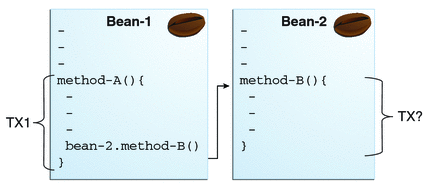
\includegraphics[scale=.7]{img/obr3}
\end{frame}



\begin{frame}[fragile]\frametitle{EJB Transactions}
  \begin{itemize}
  	\item Bean-managed
    \begin{itemize}
    	\item[]
        	\begin{Verbatim}[fontsize=\footnotesize, commandchars=\\\{\}]
@TransactionManagement(TransactionManagementType.BEAN)
\textcolor{purple}{\textbf{class}} MyBean \{ \ldots 

    @Resource
    UserTransaction userTransaction;

    \ldots
    userTransaction.begin();
    \ldots
    \ldots
    userTransaction.commit();
    userTransaction.rollback();
    \ldots
\}
            \end{Verbatim}
    \end{itemize}
  \end{itemize}
\end{frame}


\begin{frame}\frametitle{EJB Lite}
	\begin{itemize}
		\item EJB Lite is a subset of the full EJB.
		\item EJB Lite can be a part of .war file.
        \item A Java EE Web Profile certified container has to support the EJB Lite.
		\item A subset of EJB Full
          \begin{itemize}
        	\item no Message Driven Beans
        	\item no remote interfaces
        	\item no EJB timers and scheduling
        	\item no asynchronous invocation
        	\item no web services
          \end{itemize}
	\end{itemize}
\begin{tikzpicture}[remember picture,overlay]
    \node[xshift=-0.6cm,yshift=-1.3cm] at (current page.north east){%
    
\includegraphics[width=1cm]{img/oko}};
\end{tikzpicture}
\end{frame}


\begin{frame}[fragile]\frametitle{Embeddable Container}
	\begin{itemize}
		\item Client and EJB runs on the same JVM.
		\item Better support for testing.
		\item Batch processing.
		\item Usage of EJB programming model in desktop applications.
		\item[]
        	\medskip
            \begin{Verbatim}[fontsize=\footnotesize, commandchars=\\\{\}]
@Test
\textcolor{purple}{\textbf{public void}} hello() \textcolor{purple}{\textbf{throws}} Exception \{
    EJBContainer ec = EJBContainer.createEJBContainer();
    Context c = ec.getContext();
    HelloSessionBean hello = (HelloSessionBean)
       c.lookup( \textcolor{blue}{"java:global/classes/HelloSessionBean"} );
    \textcolor{purple}{\textbf{String}} s = hello.sayHello( \textcolor{blue}{"Eva"} );
    assertEquals( \textcolor{blue}{"Hello, Eva"}, s );
\}
			\end{Verbatim}
	\end{itemize}
\begin{tikzpicture}[remember picture,overlay]
    \node[xshift=-0.6cm,yshift=-1.3cm] at (current page.north east){%
    
\includegraphics[width=1cm]{img/oko}};
\end{tikzpicture}
\end{frame}


\begin{frame}\frametitle{Contents of EJB}
	\begin{multicols}{2}
		\begin{itemize}
			\item Enterprise bean class
			\item Business interfaces
			\item Other classes
			\item Deployment descriptor (optional)
		\end{itemize}
        \vfill
    \columnbreak
        \vfill
        \putat{-25}{-140}{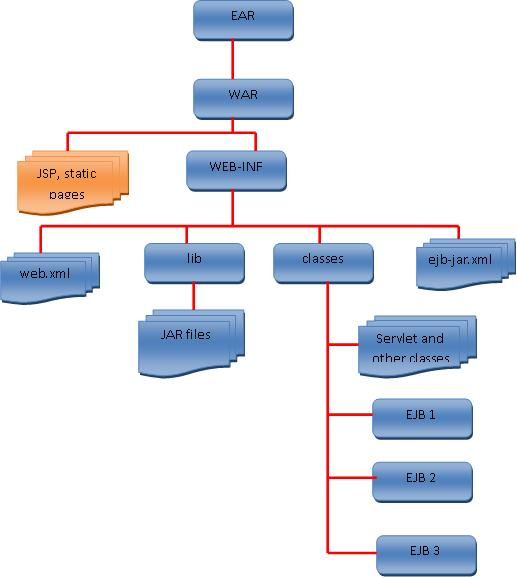
\includegraphics[scale=0.5]{img/obr4}}
	\end{multicols}
\end{frame}


\begin{frame}\frametitle{Deployment Descriptors}
	\begin{itemize}
        \item Deployment Descriptors are included in the JARs, along with component-related resources.
        \item Deployment Descriptors are XML documents that describe configuration and other deployment settings.
        \item The statements in the deployment descriptor are declarative instructions to the Java EE container (transactional settings, \ldots).
        \item The deployment descriptor for an EJB component must be named \texttt{ejb-jar.xml}, and it resides in the META-INF directory inside the EJB JAR files.
        \item It is also possible to configure it using annotations.
	\end{itemize}
\end{frame}


\begin{frame}\frametitle{References}
	\begin{itemize}
		\item JSR-299 (CDI)
          \begin{itemize}
        	\item[] {\footnotesize\url{http://docs.jboss.org/weld/reference/latest/en-US/html/}}
          \end{itemize}
		\item Java EE 6 Tutorial
          \begin{itemize}
        	\item[] {\footnotesize\url{https://docs.oracle.com/javaee/6/tutorial/doc/}}
          \end{itemize}
            \item Jakarta EE Tutorial
          \begin{itemize}
              \item \url{https://eclipse-ee4j.github.io/jakartaee-tutorial/}
          \end{itemize}
        \item Oracle\textregistered{} Containers for J2EE Enterprise JavaBeans Developer's Guide
          \begin{itemize}
            \item[] {\footnotesize\url{https://docs.oracle.com/cd/E16439_01/doc.1013/e13981/toc.htm}}
          \end{itemize}
        \item Programming WebLogic Enterprise JavaBeans
          \begin{itemize}
            \item[] {\footnotesize\url{https://docs.oracle.com/cd/E13222_01/wls/docs81/ejb/session.html}}
          \end{itemize}
        \item Simplify enterprise Java development with EJB 3.0, Part 1
          \begin{itemize}
            \item[] {\footnotesize\url{https://www.javaworld.com/article/2072037/java-web-development-simplify-enterprise-java-development-with-ejb-3-0-part-1.html}}
          \end{itemize}
	\end{itemize}
\end{frame}

\begin{frame}\frametitle{References}
	\begin{itemize}
            \item Distributed Multitiered Applications -- Tiers
          \begin{itemize}
            \item \url{https://docs.oracle.com/javaee/6/tutorial/doc/bnaay.html}
          \end{itemize}
		\item The Open Tutorials - Java EE
          \begin{itemize}
        	\item[] {\footnotesize\url{http://theopentutorials.com/content/tutorials/java-ee/}}
          \end{itemize}
        \item Stateful session beans (EJB 3)
         \begin{itemize}
        	\item[] {\footnotesize\url{http://vkpedia.com/sandbox/files/EJB\%203\%20in\%20Action.pdf}}
          \end{itemize}
        \item Others
          \begin{itemize}
            \item \url{https://access.redhat.com/solutions/158153}
          \end{itemize}
	\end{itemize}
\end{frame}

\bluepage{JavaServer Faces}

\begin{frame}\frametitle{Contents}
  \begin{itemize}
    \item Introduction
    \item Creating pages and backing beans (dynamic binding with EL)
    \item Defining navigation
    \item JSF Lifecycle
    \item Data Conversion and Validation
    \item Events
    \item Other frameworks (PrimeFaces)
    \item Conclusions
  \end{itemize}
\end{frame}


\begin{frame}\frametitle{Introduction}
	\begin{itemize}
		\item JavaServer Faces (JSF)
          \begin{itemize}
        	\item application framework for creating Web-based user interfaces
        	\item component-based
        	\item provides standard set of components
        	\item transparently saves and restores component state
        	\item event handling, server side validation, data conversion
        	\item framework for implementing custom components
            \medskip
            \item based on Model-View-Controller (MVC) 
            \item running in the standard web container (e.g. Tomcat or Jetty)
          \end{itemize}
	\end{itemize}
\begin{tikzpicture}[remember picture,overlay]
    \node[xshift=-0.6cm,yshift=-1.3cm] at (current page.north east){%
    
\includegraphics[width=1cm]{img/oko}};
\end{tikzpicture}
\end{frame}


\begin{frame}\frametitle{JSF application}
	\begin{itemize}
        \item JSF tags in a Java Server Pages (JSP) files (\texttt{.jsp}) 
    or in facelets (\texttt{.xhtml})
            \begin{itemize}
                \item defines the layout of JSF components
            \end{itemize}
        \item Backing beans (\texttt{.java})
            \begin{itemize}
                \item JavaBeans components, defines properties and functions for UI components on a page
            \end{itemize}
        \item Configuration resource files (\texttt{web.xml}, \texttt{faces-config.xml})
            \begin{itemize}
                \item navigation, configuration of backing beans, custom components, deployment descriptor
            \end{itemize}
        \item Custom objects (\texttt{.java})
            \begin{itemize}
                \item Custom UI components, validators, converters, listeners
            \end{itemize}
        \item Custom tag library definition (\texttt{.xml})
	\end{itemize}
\begin{tikzpicture}[remember picture,overlay]
    \node[xshift=-0.6cm,yshift=-1.3cm] at (current page.north east){%
    
\includegraphics[width=1cm]{img/lupa}};
\end{tikzpicture}
\end{frame}


\begin{frame}\frametitle{JSF Architecture}
\begin{center}
  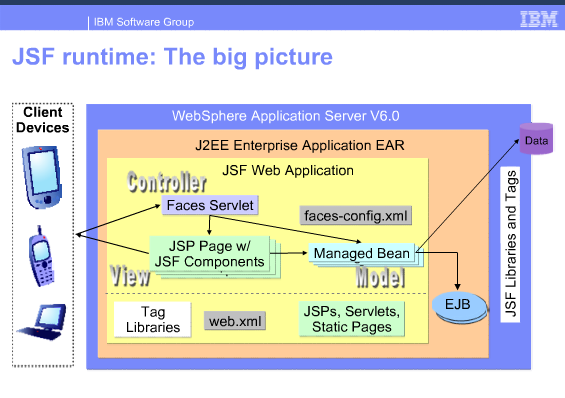
\includegraphics[scale=0.55]{img/obr5}
\end{center}
\end{frame}


\begin{frame}\frametitle{JSF Lifecycle}
\begin{itemize}
  \item JSF manages components' state
\end{itemize}
\begin{center}
  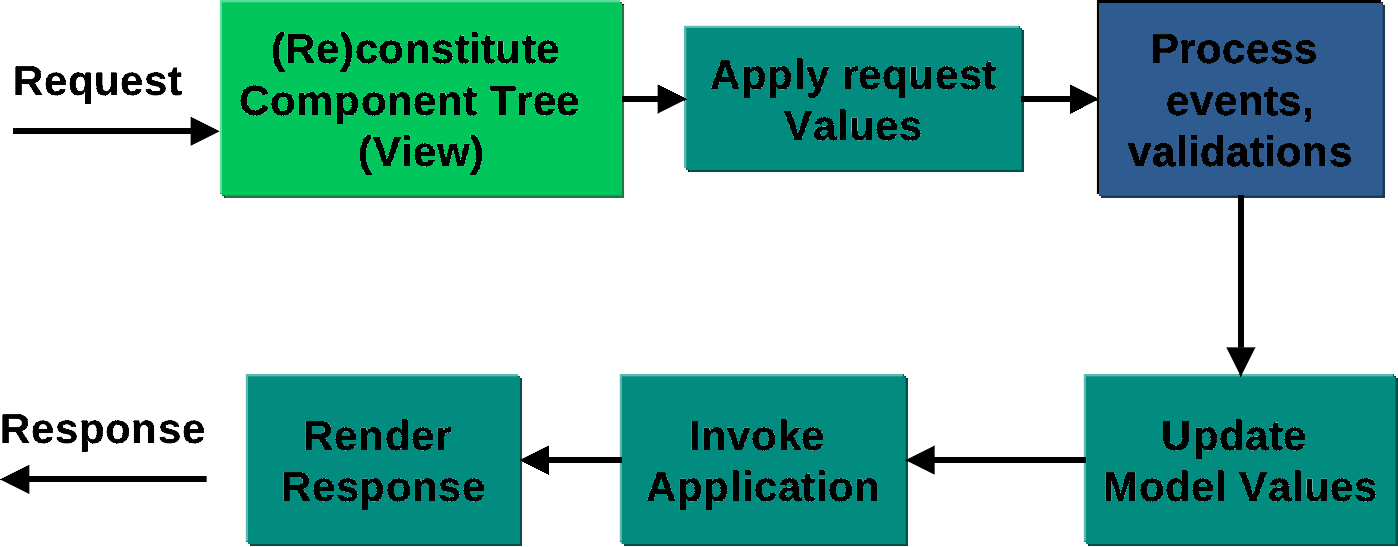
\includegraphics[scale=0.23]{img/obr6}
\end{center}
\begin{tikzpicture}[remember picture,overlay]
    \node[xshift=-0.6cm,yshift=-1.3cm] at (current page.north east){%
    
\includegraphics[width=1cm]{img/pozor}};
\end{tikzpicture}
\end{frame}


\begin{frame}\frametitle{1. (Re)Constitute component tree}
	\begin{itemize}
		\item ID of the view is extracted from the request \\(name of the page).
		\item Component tree for the current view is created.
		\item Two possibilities
          \begin{itemize}
        	\item initial request
              \begin{itemize}
            	\item build a view of the page (ui components), event handlers, validators, \ldots
              \end{itemize}
            \item postback
              \begin{itemize}
                \item form was sent
            	\item restore view from state information (server or client)
              \end{itemize}
          \end{itemize}
	\end{itemize}
\begin{tikzpicture}[remember picture,overlay]
    \node[xshift=-0.6cm,yshift=-1.3cm] at (current page.north east){%
    
\includegraphics[width=1cm]{img/pozor}};
\end{tikzpicture}
\end{frame}


\begin{frame}\frametitle{2. Apply Request Values}
	\begin{itemize}
		\item Every component retrieves current state.
		\item Calls the decode method on component renderer
          \begin{itemize}
        	\item set component values, queue events, messages
            \item values from request (headers, cookies, form data)
          \end{itemize}
        \item If any decode methods / event listeners called \texttt{renderResponse} on the current \texttt{FacesContext} instance, the JSF moves to the render response phase.
        \medskip
        \item Values are converted from strings and set into instances of UI component classes.
	\end{itemize}
\begin{tikzpicture}[remember picture,overlay]
    \node[xshift=-0.6cm,yshift=-1.3cm] at (current page.north east){%
    
\includegraphics[width=1cm]{img/pozor}};
\end{tikzpicture}
\end{frame}


\begin{frame}\frametitle{3. Process events, validations}
      \begin{itemize}
          \item Queued events processed after Apply Request Phase.
          \item Processes all validators registered on the components in the tree
            \begin{itemize}
              \item validators may \texttt{setValid(false) }
              \item error message added to \texttt{FacesContext}
              \item if any validation error, skip to Render Response phase
              \item otherwise, continue to the Update Model Values Phase.
            \end{itemize}
          \item If the local value is invalid, the JSF adds an error message to the \texttt{FacesContext} instance, and the life cycle advances to the Render Response phase and display the same page again with the error message.
            \begin{itemize}
              \item \texttt{FacesContext} contains objects on the page.
            \end{itemize}
      \end{itemize}
\begin{tikzpicture}[remember picture,overlay]
    \node[xshift=-0.6cm,yshift=-1.3cm] at (current page.north east){%
    
\includegraphics[width=1cm]{img/pozor}};
\end{tikzpicture}
\end{frame}


\begin{frame}\frametitle{4. Update Model Values}
	\begin{itemize}
		\item Updates values of the model (properties of the managed beans).
		\item Conversion errors may happen.
		\item If any \texttt{updateModels} methods or any listeners called \texttt{renderResponse} on the current \texttt{FacesContext} instance, the JSF moves to the Render Response phase.
	\end{itemize}
\begin{tikzpicture}[remember picture,overlay]
    \node[xshift=-0.6cm,yshift=-1.3cm] at (current page.north east){%
    
\includegraphics[width=1cm]{img/pozor}};
\end{tikzpicture}
\end{frame}


\begin{frame}\frametitle{5. Invoke Application}
	\begin{itemize}
		\item Handles any application-level events, such as submitting of a~form or linking to another page.
		\item Application may define a next view
          \begin{itemize}
            \item action event (form submission).
        	\item default \texttt{ActionListener} handles the ``action'' result and passes to \texttt{NavigationHandler}.
            \item Value of \texttt{action} in \texttt{UICommand} is compared with the rules in the \texttt{faces-config.xml}.
          \end{itemize}
	\end{itemize}
\begin{tikzpicture}[remember picture,overlay]
    \node[xshift=-0.6cm,yshift=-1.3cm] at (current page.north east){%
    
\includegraphics[width=1cm]{img/pozor}};
\end{tikzpicture}
\end{frame}


\begin{frame}\frametitle{6. Render Response Phase}
	\begin{itemize}
		\item JSP or facelet container will render the page
          \begin{itemize}
        	\item JSF tag handlers will setup rendering of the components.
        	\item User can see the result.
          \end{itemize}
		\item After the content of the view is rendered, the response state is saved so that subsequent requests can access it and it is available to the restore view phase.
          \begin{itemize}
            \item Tags \texttt{<message/>} and \texttt{<messages/>} (for errors, etc.)
          \end{itemize}
	\end{itemize}
\begin{tikzpicture}[remember picture,overlay]
    \node[xshift=-0.6cm,yshift=-1.3cm] at (current page.north east){%
    
\includegraphics[width=1cm]{img/pozor}};
\end{tikzpicture}
\end{frame}


\begin{frame}\frametitle{JSF Lifecycle}
\begin{center}
  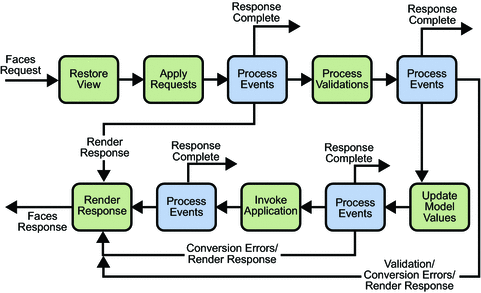
\includegraphics[scale=0.65]{img/obr7}
\end{center}
\end{frame}


\begin{frame}\frametitle{JSF Technology}
  	\quad JSF UI Components
    \medskip
	\begin{itemize}
		\item basic building blocks of a JSF application
		\item can represent simple to complex user interface components ranging from a button or input field to a~complete page
		\item can be associated to Model data objects through Value Binding
          \begin{itemize}
            \item usage of EL (\texttt{\$\{\ldots \}} and \texttt{\#\{\ldots \}})
          \end{itemize}
		\item UI Components use helper objects: validators, converters, listeners/events
	\end{itemize}
\begin{tikzpicture}[remember picture,overlay]
    \node[xshift=-0.6cm,yshift=-1.3cm] at (current page.north east){%
    
\includegraphics[width=1cm]{img/oko}};
\end{tikzpicture}
\end{frame}


\begin{frame}\frametitle{User Interface Component Classes}
	\begin{itemize}
      \item JSF components have two parts
        \begin{itemize}
        	\item Component (Java Class)
            \item Renderer (JQuery)
        \end{itemize}
      \item Displaying of component
        \begin{itemize}
        	\item Direct implementation (component encodes/decodes itself)
            \item Delegated implementation (encoding/decoding delegated to Renderer -- used for extensions)
        \end{itemize}
      \item \texttt{UIComponent}
        \begin{itemize}
        	\item form a tree, instance of \texttt{UIViewRoot} class is the root
        	\item hold state (interface \texttt{StateHolder}), registers listeners, \ldots
        \end{itemize}
      \item UI Component classes
        \begin{itemize}
        	\item \texttt{UIViewRoot, UIForm}
        	\item \texttt{UIOutput, UIInput}
        	\item \texttt{UICommand}
        	\item \texttt{UISelectMany, UISelectOne, UISelectItem}
        	\item \texttt{UIData, UIColumn}
        	\item \texttt{UIPanel}
        \end{itemize}
	\end{itemize}
\begin{textblock}{15}(10.6,0.8)
    {\footnotesize Example JSFTutorial}
\end{textblock}
\begin{tikzpicture}[remember picture,overlay]
    \node[xshift=-0.6cm,yshift=-1.3cm] at (current page.north east){%
    
\includegraphics[width=1cm]{img/oko}};
\end{tikzpicture}
\end{frame}


\begin{frame}\frametitle{Component rendering}
	\begin{itemize}
        \item Renderer
          \begin{itemize}
            \item JSF tree to HTML (XUL, SVG, \ldots)
          \end{itemize}
		\item Renderkit
          \begin{itemize}
        	\begin{footnotesize}
              \item set of renderers with same output format
              \item multiple renderers for one component
                \begin{itemize}
                  \begin{scriptsize}        
                      \item \texttt{UICommand} -- \texttt{commandLink}, \texttt{commandButton}
                      \item \texttt{UISelectOne} -- \texttt{selectOneListbox}, \texttt{selectOneMenu}, \texttt{selectOneRadio}
                  \end{scriptsize}
                \end{itemize}
              \item defined in tag library
            \end{footnotesize}
          \end{itemize}
		\item Component tags
          \begin{itemize}
        	{\footnotesize\item \texttt{outputText, inputText, inputTextarea, inputHidden, inputSecret,} \ldots}
          \end{itemize}
		\item Component tag attributes
          \begin{itemize}
        	\begin{footnotesize}
              \item \texttt{id}: unique id of the component
              \item \texttt{immediate}: events, validation, conversion should	happen in the ``apply request phase'' -- use this attribute to skip validation in case of Cancel button is clicked. 
              \item \texttt{rendered}: do not render if set to false
              \item \texttt{value}: binds the value to some backing bean property
              \item \texttt{binding}: binds the instance to some backing bean property (whole component!)
              \item \texttt{style}
              \item \texttt{styleClass}
        	\end{footnotesize}
          \end{itemize}
	\end{itemize}
\begin{tikzpicture}[remember picture,overlay]
    \node[xshift=-0.6cm,yshift=-1.3cm] at (current page.north east){%
    
\includegraphics[width=1cm]{img/lupa}};
\end{tikzpicture}
\end{frame}


\begin{frame}[fragile]\frametitle{Creating pages}
    \begin{itemize}
      	\item JSP pages with JSF tag library
      	\item View is a tree of JSF components
      	\item Editable components inside a ``form'' component
        \item[]
        	\medskip
            \begin{Verbatim}[fontsize=\scriptsize, commandchars=\\\{\}]
<%@ taglib uri="http://xmlns.jcp.org/jsf/html" prefix="h" %>
<%@ taglib uri="http://xmlns.jcp.org/jsf/core" prefix="f" %>
<f:view>
  <h:form id="signinForm">
    <h:inputText id="name" value="#{SigninBean.name}" required="true"/>
    <h:commandButton id="submit" action="#{SigninBean.signin}"
    	         value="Submit" />
  </h:form>
</f:view>           
            \end{Verbatim}
    \end{itemize}
\end{frame}


\begin{frame}[fragile]\frametitle{Backing beans}
	\begin{itemize}
		\item Usually one managed bean per page.
		\item Backing beans defines properties and methods associated with UI components.
		\item Component value to bean property binding defined in JSF page using Unified Expression Language (EL)
		\item[]
        	\medskip
            \begin{Verbatim}[fontsize=\scriptsize, commandchars=\\\{\}]
\textcolor{purple}{\textbf{class}} SigninBean \{
    \textcolor{purple}{\textbf{private String}} name;
    \textcolor{purple}{\textbf{public String}} getName() \{ \textcolor{purple}{\textbf{return}} name; \} 
    \textcolor{purple}{\textbf{public void}} setName(\textcolor{purple}{\textbf{String}} name) \{ \textcolor{purple}{\textbf{this}}.name = name; \}
    \textcolor{purple}{\textbf{public String}} signin() \{
        \ldots
        \textcolor{purple}{\textbf{if}} (ok) \{ \textcolor{purple}{\textbf{return}} \textcolor{blue}{"success"}; \} \textcolor{purple}{\textbf{else}} \{ \textcolor{purple}{\textbf{return null}}; \}
    \}
\}
			\end{Verbatim}
	\end{itemize}
\begin{tikzpicture}[remember picture,overlay]
    \node[xshift=-0.6cm,yshift=-1.3cm] at (current page.north east){%
    
\includegraphics[width=1cm]{img/oko}};
\end{tikzpicture}
\end{frame}


\begin{frame}\frametitle{JSF Managed Beans}
	\begin{itemize}
		\item JSF Managed Beans works as Model for UI component,
        \item can be acessed from JSF page,
        \item contains getters, setters (like backing bean),
          \begin{itemize}
            \item {\footnotesize Backing bean contains all the HTML form values, managed not.}
          \end{itemize}
        \item registered through annotations
          \begin{itemize}
            \item {\footnotesize \texttt{@ManagedBean(name="helloWorld", eager=true)}}
              \begin{itemize}
                \item {\footnotesize \texttt{eager=true} -- created before requested, otherwise lazy}
              \end{itemize}
          \end{itemize}
        \item Scopes
        \item[] \texttt{@RequestScoped, @NoneScoped, @ViewScoped, @SessionScoped, @ApplicationScoped, @CustomScoped}
          \begin{itemize}
              \item \texttt{@NoneScoped} created on every single EL expression referencing the bean.
          \end{itemize}
        \item \texttt{@ManagedProperty} annotation
        \begin{itemize}
            \item {\footnotesize Bean can be injected to another managed bean.}
        \end{itemize}
	\end{itemize}
\begin{tikzpicture}[remember picture,overlay]
    \node[xshift=-0.6cm,yshift=-1.3cm] at (current page.north east){%
    
\includegraphics[width=1cm]{img/lupa}};
\end{tikzpicture}
\end{frame}


\begin{frame}\frametitle{JSF Managed Beans}
	\begin{itemize}
      \item From JSF 2.2 it is highly recommended to use CDI (Contexts and Dependency Injection).
      \item \texttt{@ManagedBean} is deprecated
        \begin{itemize}
          \item \texttt{@Named} (\texttt{jakarta.inject.Named}) can be used instead
          \item \texttt{eager = true} needs extension \url{https://www.javacodegeeks.com/2013/02/jsf-eager-cdi-beans.html}
        \end{itemize}
      \item \texttt{javax.faces.bean.SessionScoped} is deprecated
        \begin{itemize}
          \item \texttt{jakarta.enterprise.context.SessionScoped} can be used instead
          \item similar for other scopes (e. g. \texttt{jakarta.enterprise.context.ApplicationScoped})
        \end{itemize}
	\end{itemize}
\end{frame}


\begin{frame}[fragile]\frametitle{Page navigation}
	\begin{itemize}
            \item Page navigation is defined in \texttt{faces-config.xml} file
            \item can be defined in managed beans
            \item implicit navigation
            \item set of navigation rules
              \begin{itemize}
            	\begin{footnotesize}
                    \item \texttt{from-view-id} (optional)
                    \item \texttt{navigation-case}
                      \begin{itemize}
                        \item {\footnotesize \texttt{from-outcome} -- outcome as defined in JSF page or as returned by action method}\vspace{.1cm}
                        \item[] {\footnotesize\verb'<h:commandButton action="success" value="Submit" />'}
                        \item[] {\footnotesize\verb'<h:commandButton action="#{SigninBean.signin}" '}
                        \item[] {\footnotesize\verb'                 value="Submit" />'}
                        \item It is also possible to return page name directly, but it is not recommended.
                        \item Use \texttt{<redirect/>} to switch view and redirect (change URL) instead of forward (internal forwarding -- same URL).
                      \end{itemize}
                \end{footnotesize}
              \end{itemize}
            \item[]
                \medskip
                \begin{small}
                \begin{verbatim}
<navigation-rule>
   <from-view-id>/index.jsp</from-view-id>
   <navigation-case>
       <from-outcome>success</from-outcome>
       <to-view-id>/home.jsp</to-view-id>
   </navigation-case>
</navigation-rule>
                \end{verbatim}
                \end{small}
	\end{itemize}
\begin{textblock}{10}(9.0,-1.1)
    {\footnotesize Example JSFPageNavigation}
\end{textblock}
\begin{tikzpicture}[remember picture,overlay]
    \node[xshift=-0.6cm,yshift=-1.3cm] at (current page.north east){%
    
\includegraphics[width=1cm]{img/naradi}};
\end{tikzpicture}
\end{frame}


\begin{frame}[fragile]\frametitle{Conversion}
	\begin{itemize}
    	\begin{footnotesize}
            \item Value of a component can be bound (not same as binding) to a backing bean property.
            \item Conversion to some types is automatic
              \begin{itemize}
                \item {\footnotesize e.g. \texttt{UISelectBoolean} to \texttt{boolean} or \texttt{java.lang.Boolean}}
              \end{itemize}
            \item Converter Classes
              \begin{itemize}
            	\begin{footnotesize}
                    \item \texttt{BigDecimalConverter}, \texttt{IntegerConverter}, \texttt{DoubleConverter}, \ldots
                    \item
                        \begin{verbatim}
<h:inputText value="#{bean.foo}"
converter="jakarta.faces.convert.IntegerConverter" />
\end{verbatim}
                \end{footnotesize}
              \end{itemize}
            \item \texttt{DateTimeConverter}
              \begin{itemize}
            	\begin{footnotesize}
                    \item[]
                        \begin{verbatim}
<h:outputText value="#{bean.someDate}">
    <f:convertDateTime style="full" />
</h:outputText>
\end{verbatim}
                    \item \itab{\emph{style}} \tab{full, short, medium, long}
                    \item \itab{\emph{pattern}} \tab{\uv{MM dd yyyy}}
            	\end{footnotesize}
              \end{itemize}
            \item Can be created also for custom objects.
    	\end{footnotesize}
	\end{itemize}
\begin{tikzpicture}[remember picture,overlay]
    \node[xshift=-0.6cm,yshift=-1.3cm] at (current page.north east){%
    
\includegraphics[width=0.8cm]{img/oko}};
\end{tikzpicture}
\end{frame}


\begin{frame}[fragile]\frametitle{Conversion}
	\begin{itemize}
		\item Custom converters
          \begin{itemize}
        	\item interface \texttt{Converter}
            \begin{footnotesize}
            \item[] \texttt{Object getAsObject(FacesContext, UIComponent, String)}
            \item[] \texttt{String getAsString(FacesContext, UIComponent, Object)}\\[0.1cm]
            \end{footnotesize}
			\item \texttt{f:converter}
              \begin{itemize}
            	\item registered converter
                \item[]
                	\begin{verbatim}
<h:inputText>
    <f:converter converterId="MyConverter" />
</h:inputText>		\end{verbatim}
				\vspace{.05cm}
                \item binding attribute
              \end{itemize}
			\item Converter registration in faces config
            \vspace{.1cm}
            \item[]
            	\begin{verbatim}
<converter>
    <converter-for-class>com.example.MyClass
    </converter-for-class>
    <converter-class>com.example.MyConverter
    </converter-class>
</converter>            	
            	\end{verbatim}
          \end{itemize}
	\end{itemize}
\end{frame}


\begin{frame}[fragile]\frametitle{Validation}
	\begin{itemize}
		\item Validates components data, produces an error message.
		\item Standard validators
          \begin{itemize}
        	\begin{footnotesize}
                \item \texttt{validateDoubleRange}, \texttt{validateLength}, \texttt{validateLongRange}
                \item
                    \begin{verbatim}
<h:inputSecret id="password">
    <f:validateLength minimum="8"/>
</h:inputSecret>
<h:message for="password"/>  	
                    \end{verbatim}
        	\end{footnotesize}
          \end{itemize}
        \item Custom validation
          \begin{itemize}
        	\begin{footnotesize}
                \item \verb'<h:inputText validator="#{bean.validateFoo}"/>'
                \item
                    \begin{verbatim}
public void validateFoo(FacesContext context,UIComponent
 toValidate, Object value) {
    ...
    ((UIInput)toValidate).setValid(false);
}       	
                    \end{verbatim}
                \item or implement a \texttt{Validator} interface (method \texttt{validate()} throws \texttt{ValidatorException}) and register a validator in~faces-config \ldots
                \begin{itemize}
                    \item \verb'<f:validator validatorId="MyValidator"/>'
                \end{itemize}
        	\end{footnotesize}
          \end{itemize}
	\end{itemize}
\begin{tikzpicture}[remember picture,overlay]
    \node[xshift=-0.6cm,yshift=-1.3cm] at (current page.north east){%
    
\includegraphics[width=1cm]{img/oko}};
\end{tikzpicture}
\end{frame}


\begin{frame}[fragile]\frametitle{Event and Listener}
	\begin{itemize}
		\item Action events
          \begin{itemize}
            \begin{footnotesize}
                \item clicking on buttons or links
                \item
                    \begin{verbatim}
<h:commandLink action="something">
  <f:actionListener binding="fooBean.bar"/>
</h:actionLink>\end{verbatim}
                    \begin{itemize}
                        \item \verb'public void bar(ActionEvent event);'
                    \end{itemize}
                \item \texttt{<f:setPropertyActionListener target="\#\{user.username\}" ~value="some" />}
                  \begin{itemize}
                    \item sets target property of backing bean (e.g. on click)
                  \end{itemize}
            \end{footnotesize}
          \end{itemize}
		\item Value change event
          \begin{itemize}
        	\begin{footnotesize}
                \item user changes the value of a \texttt{UIInput} component
                \item \texttt{f:valueChangeListener} tag
                \begin{itemize}
                    \item \texttt{type} -- name of the class that implements \texttt{ValueChangeListener} interface
                    \item \texttt{binding} -- EL expression which evaluates to bean instance of class implementing \texttt{ValueChangeListener}
                \end{itemize}
        	\end{footnotesize}
          \end{itemize}
        \item Data model event (interface \texttt{DataModelListener})
          \begin{itemize}
        	\begin{footnotesize}
              \item new row of a \texttt{UIData} is selected
        	\end{footnotesize}
          \end{itemize}
	\end{itemize}
\begin{textblock}{20}(1.8,0.8)
    {\footnotesize Examples JSFActionListener, JSFActionListenerCDI and JSFEventListeners}
\end{textblock}
\begin{tikzpicture}[remember picture,overlay]
    \node[xshift=-0.6cm,yshift=-1.3cm] at (current page.north east){%
    
\includegraphics[width=1cm]{img/lupa}};
\end{tikzpicture}
\end{frame}


\begin{frame}[fragile]\frametitle{Using UIData}
	\begin{itemize}
      \item \texttt{h:dataTable}
        \begin{itemize}
          \item \texttt{value} - EL expression which evaluates to:
            \begin{itemize}
              \item list/array of beans, \texttt{jakarta.faces.model.DataModel}, \texttt{java.sql.ResultSet}, \texttt{javax.sql.RowSet}, \ldots
            \end{itemize}
          \item \texttt{var} -- name of the variable which iterates through the \texttt{DataModel}
          \item \texttt{first, rows,} \ldots
        \end{itemize}
      \vspace{.25cm}
	\item[]
   		\begin{footnotesize}
    		\begin{verbatim}
<h:dataTable var="i" value="#{DataTableBean.items}">
  <h:column>
    <f:facet name="header"><h:outputText value="key"/></f:facet>
      <h:commandLink action="details" value="#{i.key}">
        <f:setPropertyActionListener 
          target="#{ItemDetailBean.item}"
          value="#{i}"/>
      </h:commandLink>
  </h:column>
  <h:column>
    <f:facet name="header">
      <h:outputText value="value"/>
    </f:facet>
    <h:outputText value="#{i.value}"/>
  </h:column>
</h:dataTable>    
\end{verbatim}
   		\end{footnotesize}
	\end{itemize}
\end{frame}


\begin{frame}\frametitle{Custom components}
	\begin{itemize}
		\item \texttt{UIComponent}
          \begin{itemize}
        	\begin{footnotesize}
                \item subclass \texttt{UIComponentBase}
                \item behavioral interfaces \texttt{StateHolder, ValueHolder, NamingContainer, EditableValueHolder, ActionSource}
                \item component family
        	\end{footnotesize}
          \end{itemize}
        \item Renderer
          \begin{itemize}
        	\begin{footnotesize}
                \item \texttt{encodeBegin} (before descendants)
                \item \texttt{encodeEnd} (after descendants)
                \item \texttt{decode} (state from request)
        	\end{footnotesize}
          \end{itemize}
        \item Tag
          \begin{itemize}
        	\begin{footnotesize}
                \item abstract class \texttt{UIComponentELTag} (values from EL API)
                \item \texttt{UIComponentBodyELTag} (processing of tag body)
                \item \texttt{getComponentType, getRendererType}
                \item sets the component properties based on attributes
        	\end{footnotesize}
          \end{itemize}
	\end{itemize}
\begin{textblock}{10}(8.3,2.1)
    {\footnotesize Example JSFCustomComponent}
\end{textblock}
\end{frame}



\begin{frame}[fragile]\frametitle{JSF AJAX}
	\begin{itemize}
		\item Using AJAX technique, JavaScript code exchanges data with server and updates parts of web page without reloading of the whole page (partial rendering).
		\item JSF Tag
          \begin{itemize}
            \item[] {\footnotesize\verb'<f:ajax execute="input-component-name"'}
            \item[]	{\footnotesize\verb'        render="output-component-name" />'}
          \end{itemize}
        \item Tag attributes
          \begin{itemize}
        	\item \texttt{disabled}
        	\item \texttt{event} (what events invokes AJAX -- \texttt{blur, keypress, click, \ldots})
        	\item \texttt{execute} (processed components -- \texttt{@all})
        	\item \texttt{immediate} (\texttt{True} -- action attribute evaluated in apply request values / \texttt{False} -- action attribute evaluated in invoke application phase)
        	\item \texttt{listener} -- what should be called during AJAX request (on~the server)
        	\item \texttt{oneerror} -- name of JavaScript function, when error in AJAX occurs
        	\item \texttt{onevent} -- JavaScript callback to handle UI event
        	\item \texttt{render} -- what should be rendered
          \end{itemize}
	\end{itemize}
\begin{textblock}{10}(11,0.3)
    {\footnotesize Example JSFAjax}
\end{textblock}
\begin{tikzpicture}[remember picture,overlay]
    \node[xshift=-0.6cm,yshift=-1.3cm] at (current page.north east){%
    
\includegraphics[width=1cm]{img/oko}};
\end{tikzpicture}
\end{frame}


\begin{frame}\frametitle{Frameworks on top of JSF}
	\begin{itemize}
		\item Apache MyFaces
          \begin{itemize}
        	\item Implementation of JSF with additional components
        	\item UI-Component Sets 
              \begin{itemize}
                \item Trinidad
                \item Tobago
              \end{itemize}
          \end{itemize}
		\item ICEFaces (ICEsoft Technologies) and RichFaces (Red Hat)
          \begin{itemize}
        	\item AJAX components without writing JavaScript code
        	\item skinable
        	\item Menus, Trees, Calendar, File Upload, Drag and Drop, Google Maps, \ldots
        	\item Rich text editor
              \begin{itemize}
            	\item TinyMCE in RichFaces
            	\item CKEditor in ICEFaces
              \end{itemize}
          \end{itemize}
		\item PrimeFaces (PrimeTek Informatics)
		\item Others
	\end{itemize}
\end{frame}


\begin{frame}\frametitle{Conclusion}
	\begin{itemize}
		\item JavaServer Faces is a standard EE component based framework.
		\item JSF by default uses JSP for rendering, provides basic HTML-based components (facelets are replacing JSPs).
		\item Managed beans as backing beans for pages defines properties and methods.
		\item View state is stored between requests.
		\item Rich frameworks on top of JSF. 
	\end{itemize}
\end{frame}


\begin{frame}\frametitle{References}
	\begin{itemize}
		\item JSF
          \begin{itemize}
        	\item \url{http://www.tutorialspoint.com/jsf/}
          \end{itemize}
        \item API
          \begin{itemize}
            \item \url{http://docs.oracle.com/javaee/6/api/}
            \item \url{https://jakarta.ee/specifications/platform/10/apidocs/}
            \item \url{https://eclipse-ee4j.github.io/jakartaee-tutorial/}
          \end{itemize}
        \item Others
          \begin{itemize}
            \item \url{https://www.mkyong.com/jsf2/jsf-page-forward-vs-page-redirect/}
            \item \url{https://jakarta.ee/xml/ns/jakartaee/#10}
          \end{itemize}
	\end{itemize}
\end{frame}


\begin{frame}\frametitle{Appendix -- parameter encoding}
	\begin{itemize}
		\item GlassFish AS have deployment descriptor \texttt{glassfish-web.xml} (see \href{https://javaee.github.io/glassfish/doc/5.0/application-deployment-guide.pdf}{documentation})
        \item For correct reading of the form values with diacritic, it is necessary to set:
        \item[] \texttt{<parameter-encoding default-charset="UTF-8" />}
	\end{itemize}
\end{frame}

\bluepage{Thank you for your attention!}



\end{document}
